\documentclass[12pt]{article}
\usepackage[polish]{babel}
\usepackage[utf8]{inputenc}
\usepackage{tikz}
\usetikzlibrary{trees}
\usepackage{graphicx}
\graphicspath{ {./images/} }
\begin{document}

\begin{flushright}

Laboratoria: piatek, 8:00

Grupa: 13

Informatyka Wydział informatyki i telekomunikacji.

\end{flushright}

\hspace{4cm}

\begin{center}

Algorytmy i Strukrury Danych

Prowadzacy:

Dominik Witczak

\end{center}

\hspace{4cm}

\begin{center}

\textbf{Sprawozdanie do \LARGE}

\hspace{2cm}

\underline{Projektu 3 Sortowanie topologiczne}

\end{center}

\hspace{30cm}

\begin{flushright}

Autor:

Marcin Wrzaskowski

nr indeksu:

160329

\end{flushright}

\pagebreak

\section{Prezentacja programu: }

\subsection{Tworzenie grafów:}

\begin{center}

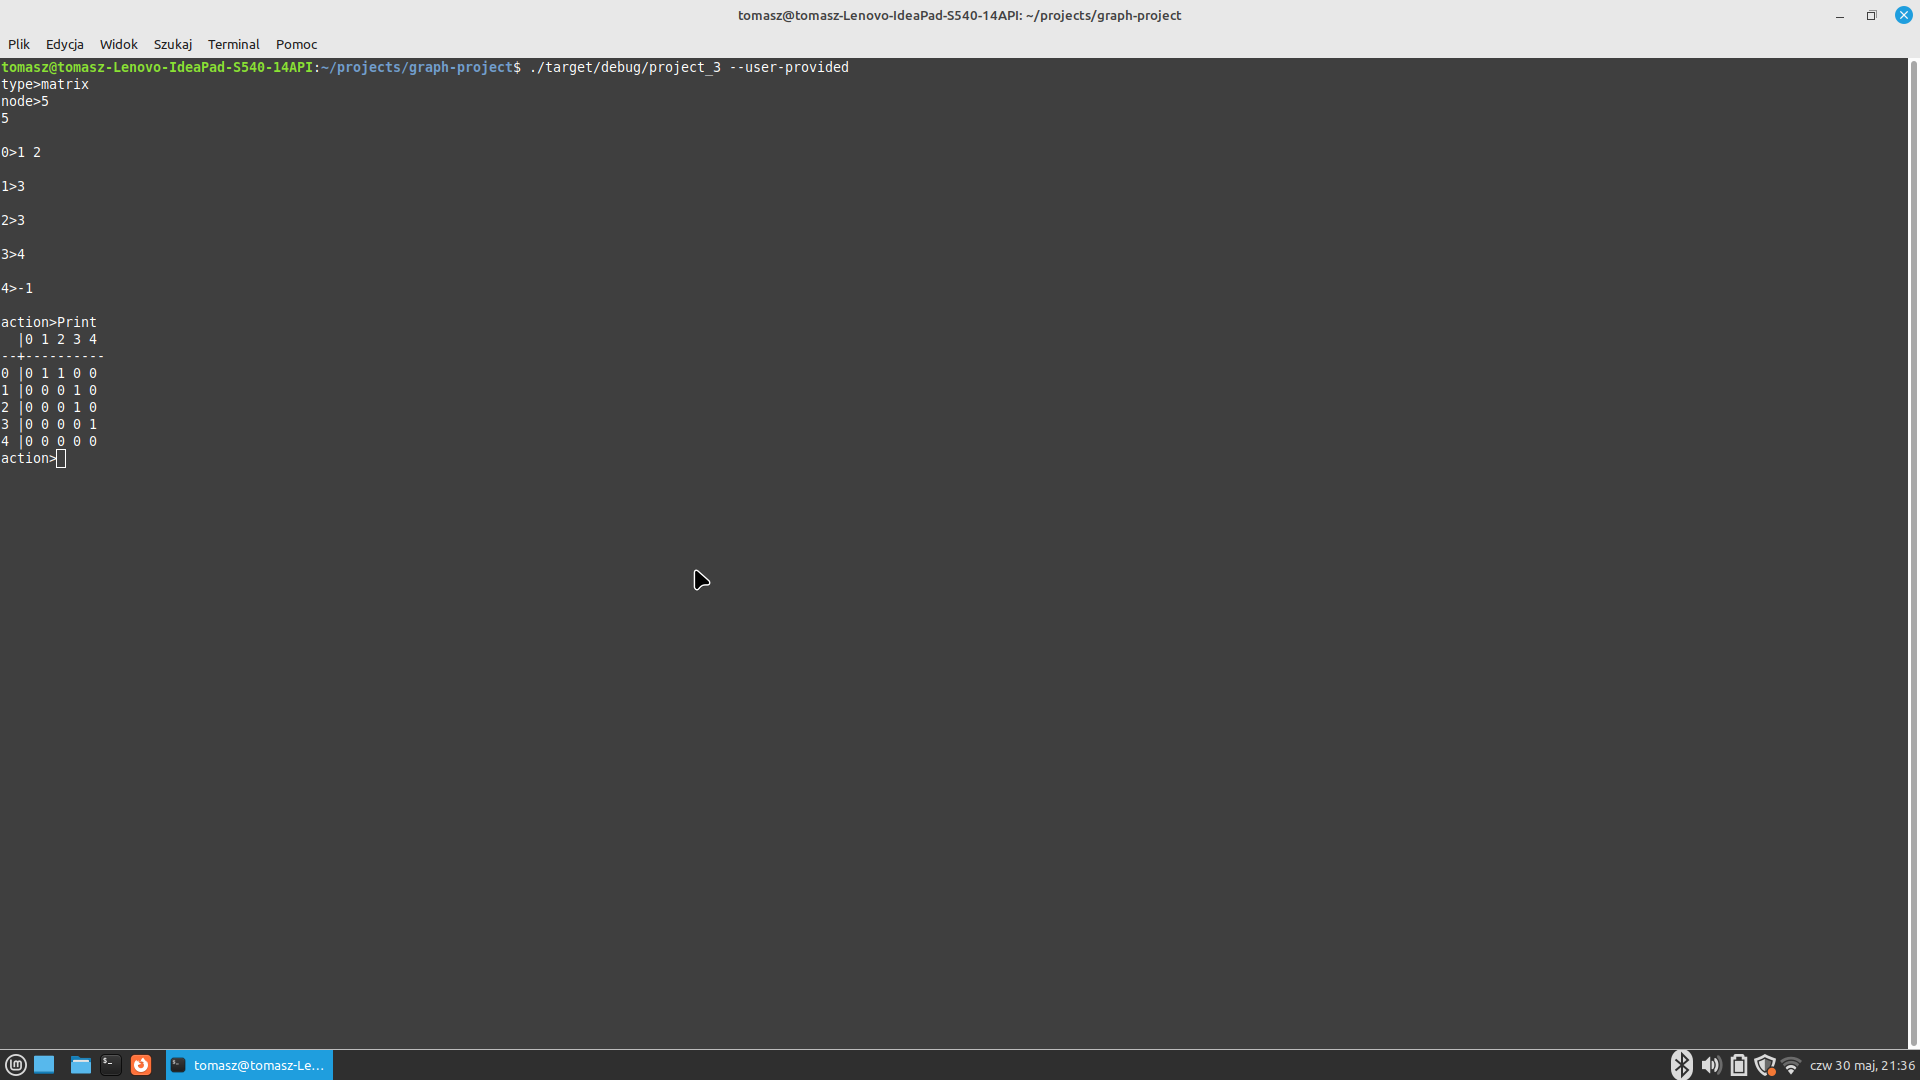
\includegraphics[scale=0.2]{matrix_graph.png}
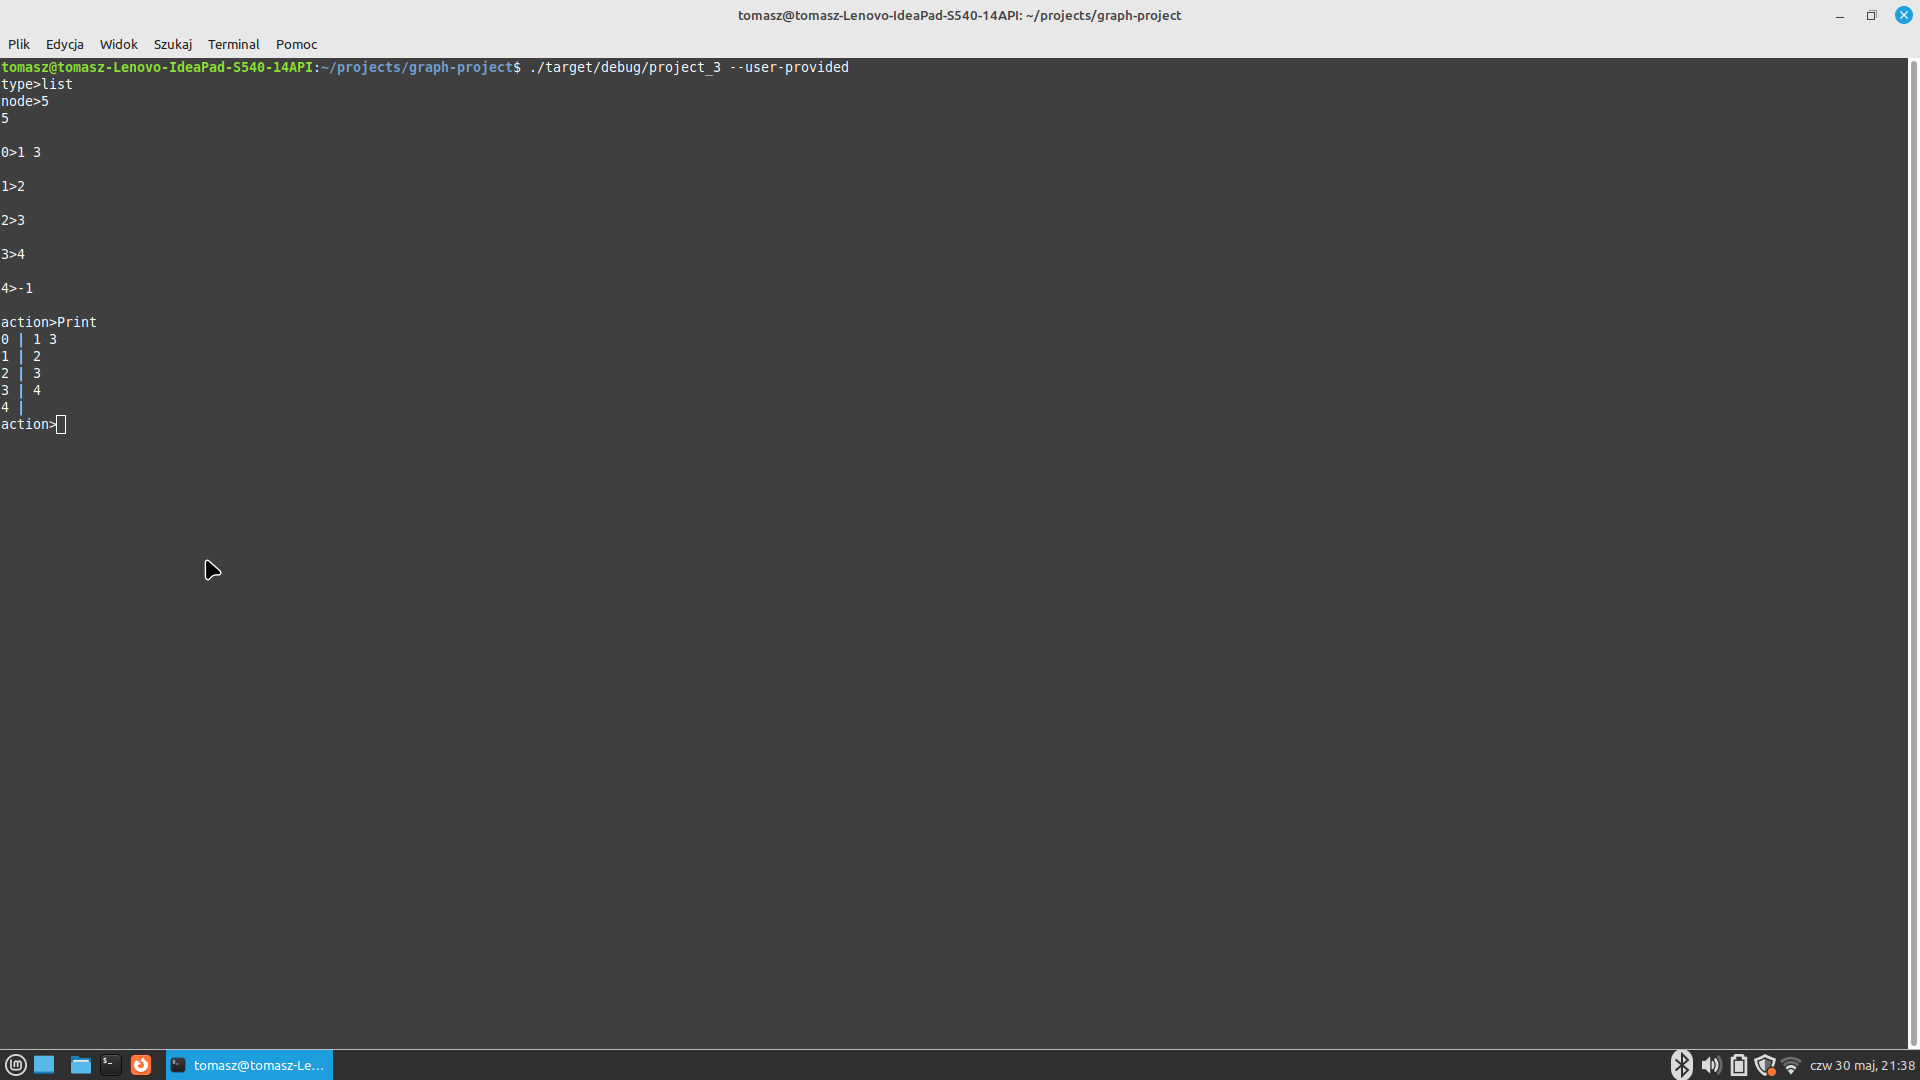
\includegraphics[scale=0.2]{list_graph.png}
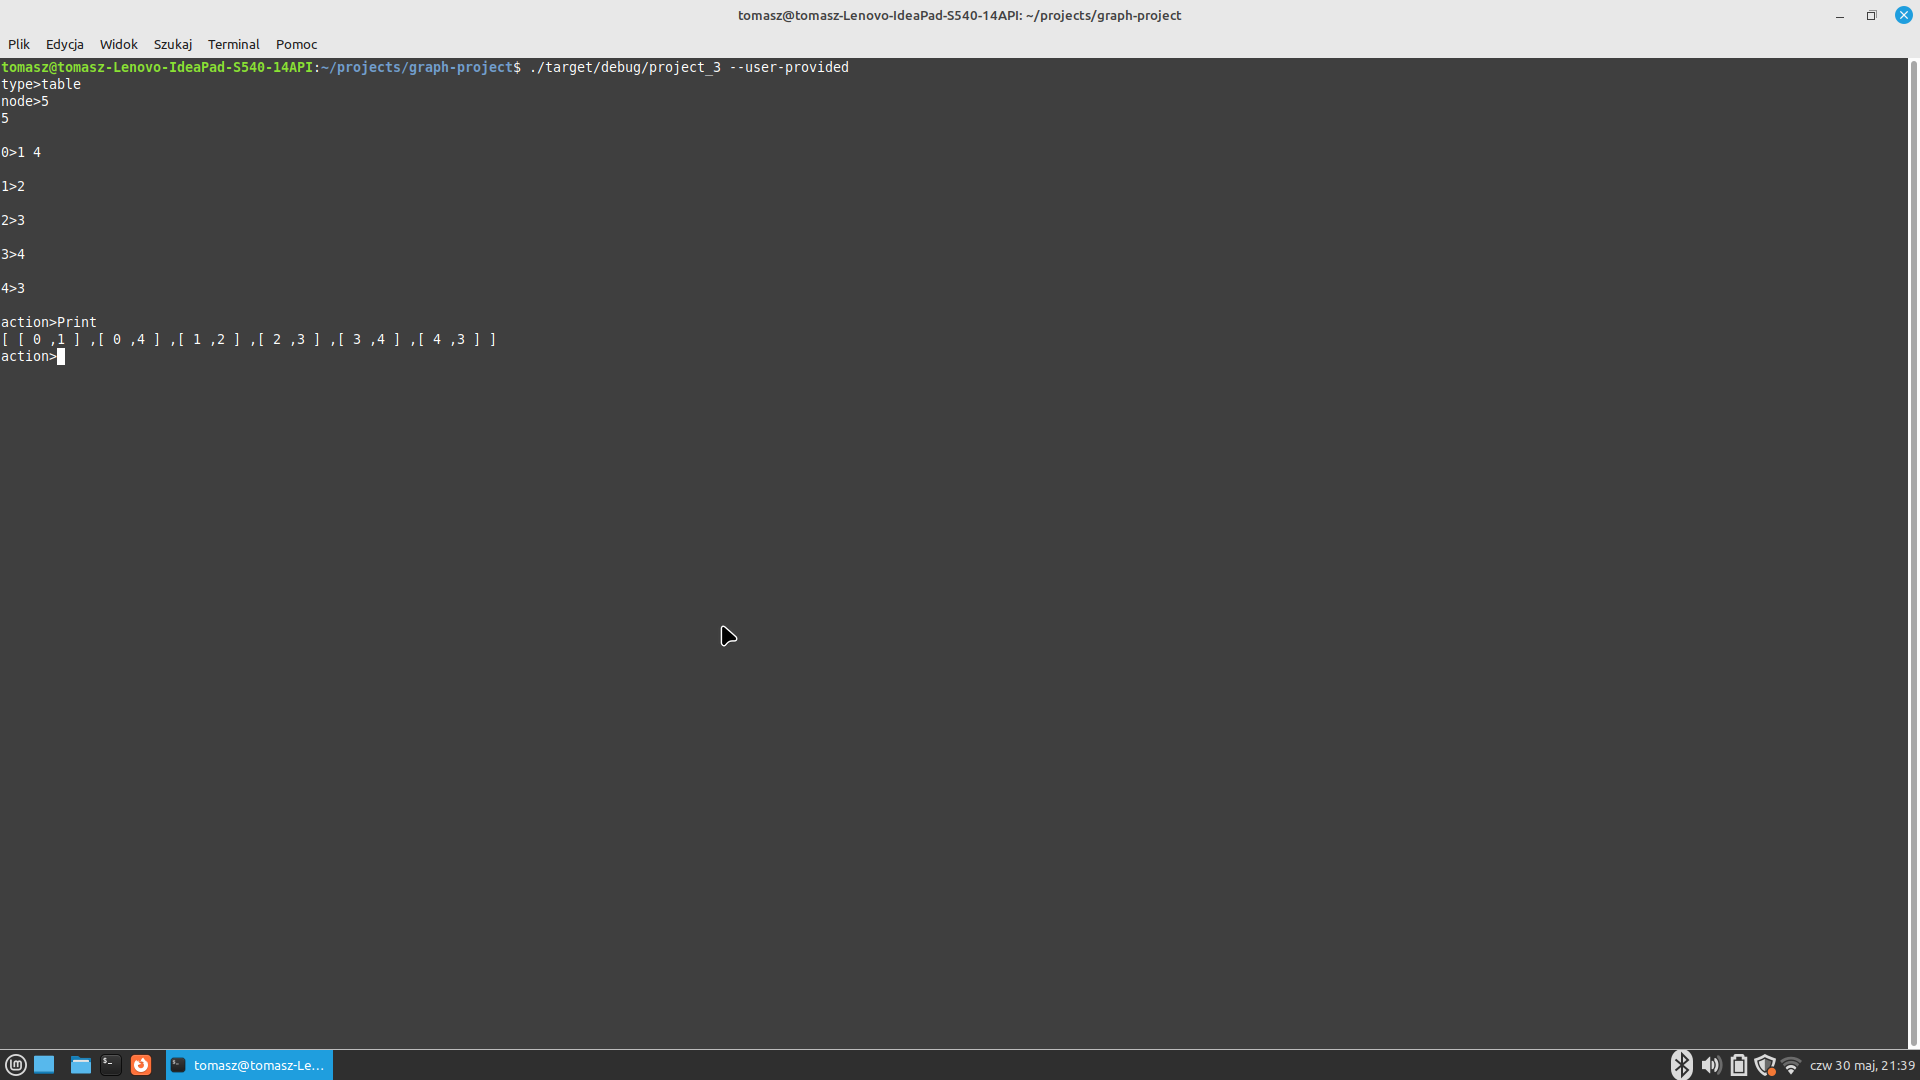
\includegraphics[scale=0.2]{table_graph.png}

\end{center}

\subsection{Wizualizacje utworzonych grafów: }

\begin{center}

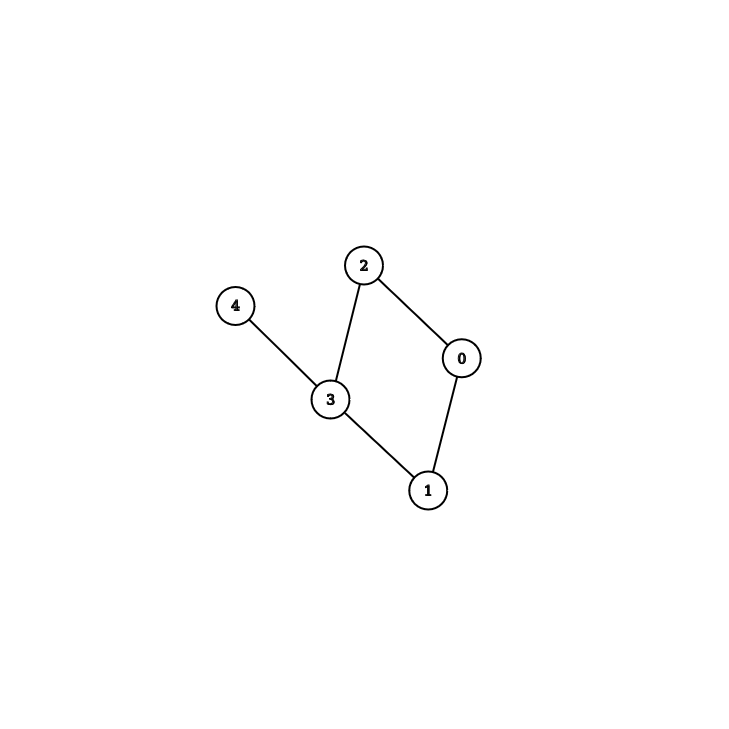
\includegraphics[scale=0.25]{graph_matrix.png}	 
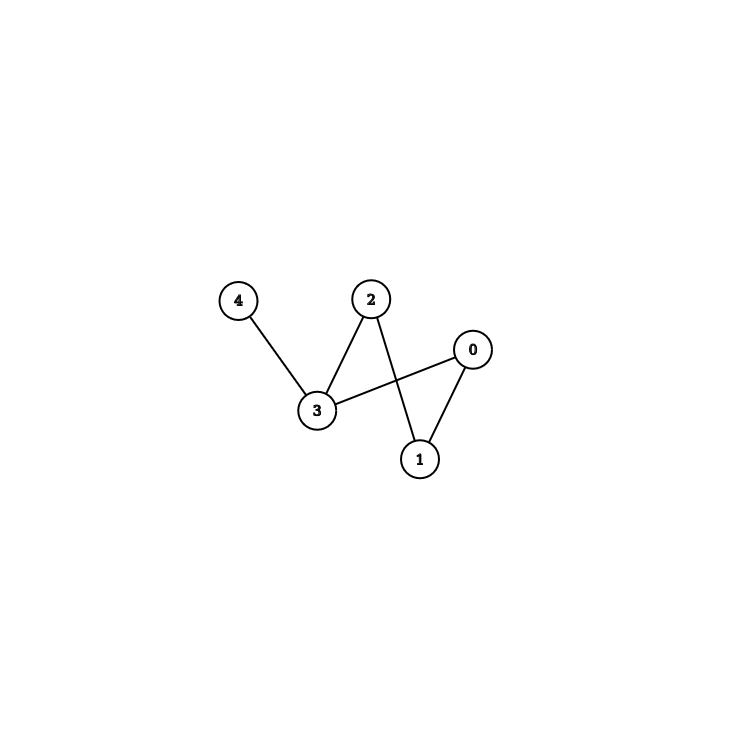
\includegraphics[scale=0.25]{graph_list.png}
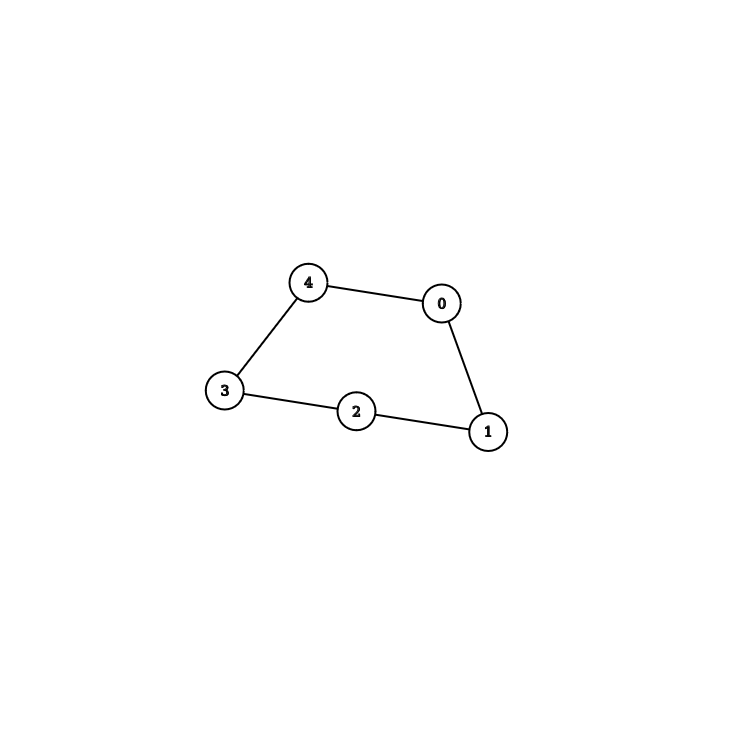
\includegraphics[scale=0.25]{graph_table.png}

\end{center}

\section{Wykresy zależności $ t = f(n) $}

\subsection{Skala liniowa: }

\begin{center}

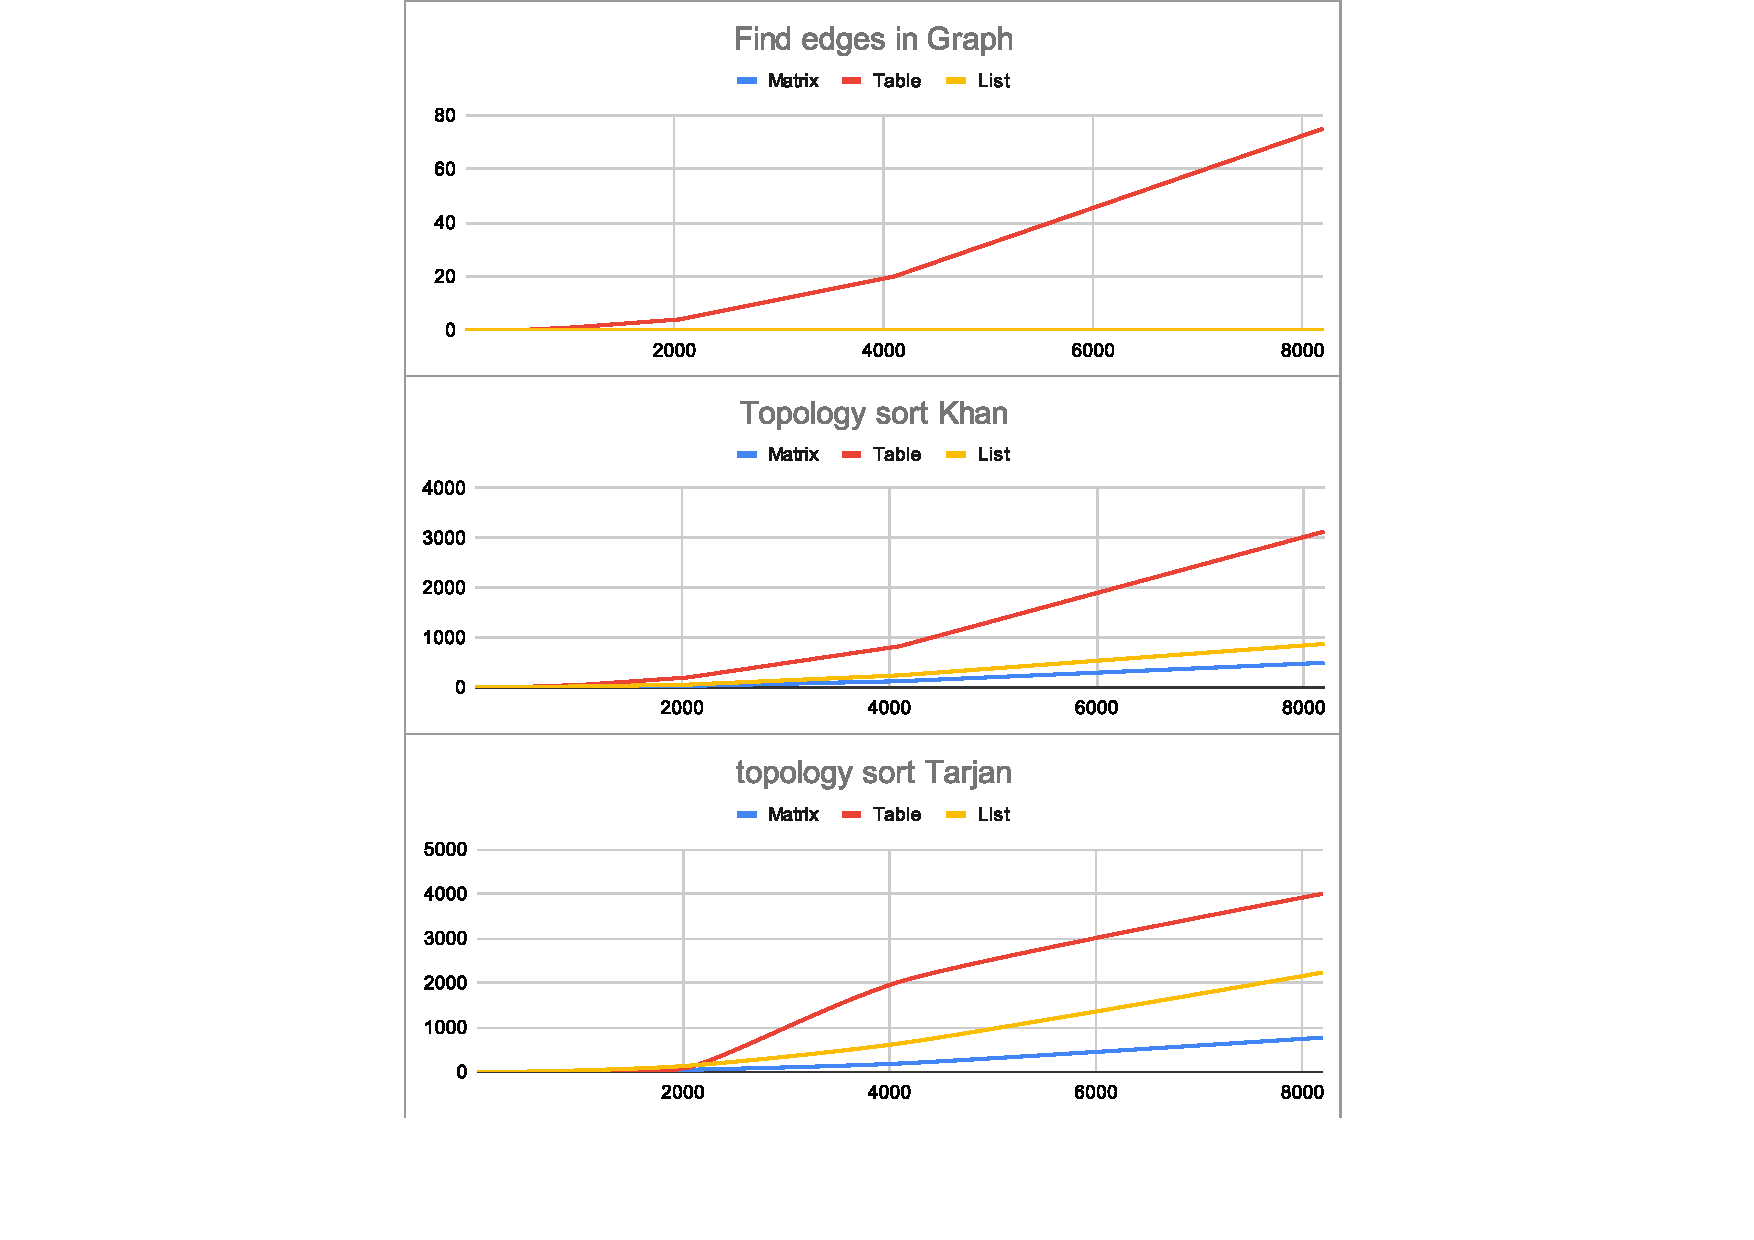
\includegraphics[width=\linewidth]{wykresy_liniowe.pdf}

\end{center}

\subsection{Skala logarytmiczna: }

\begin{center}

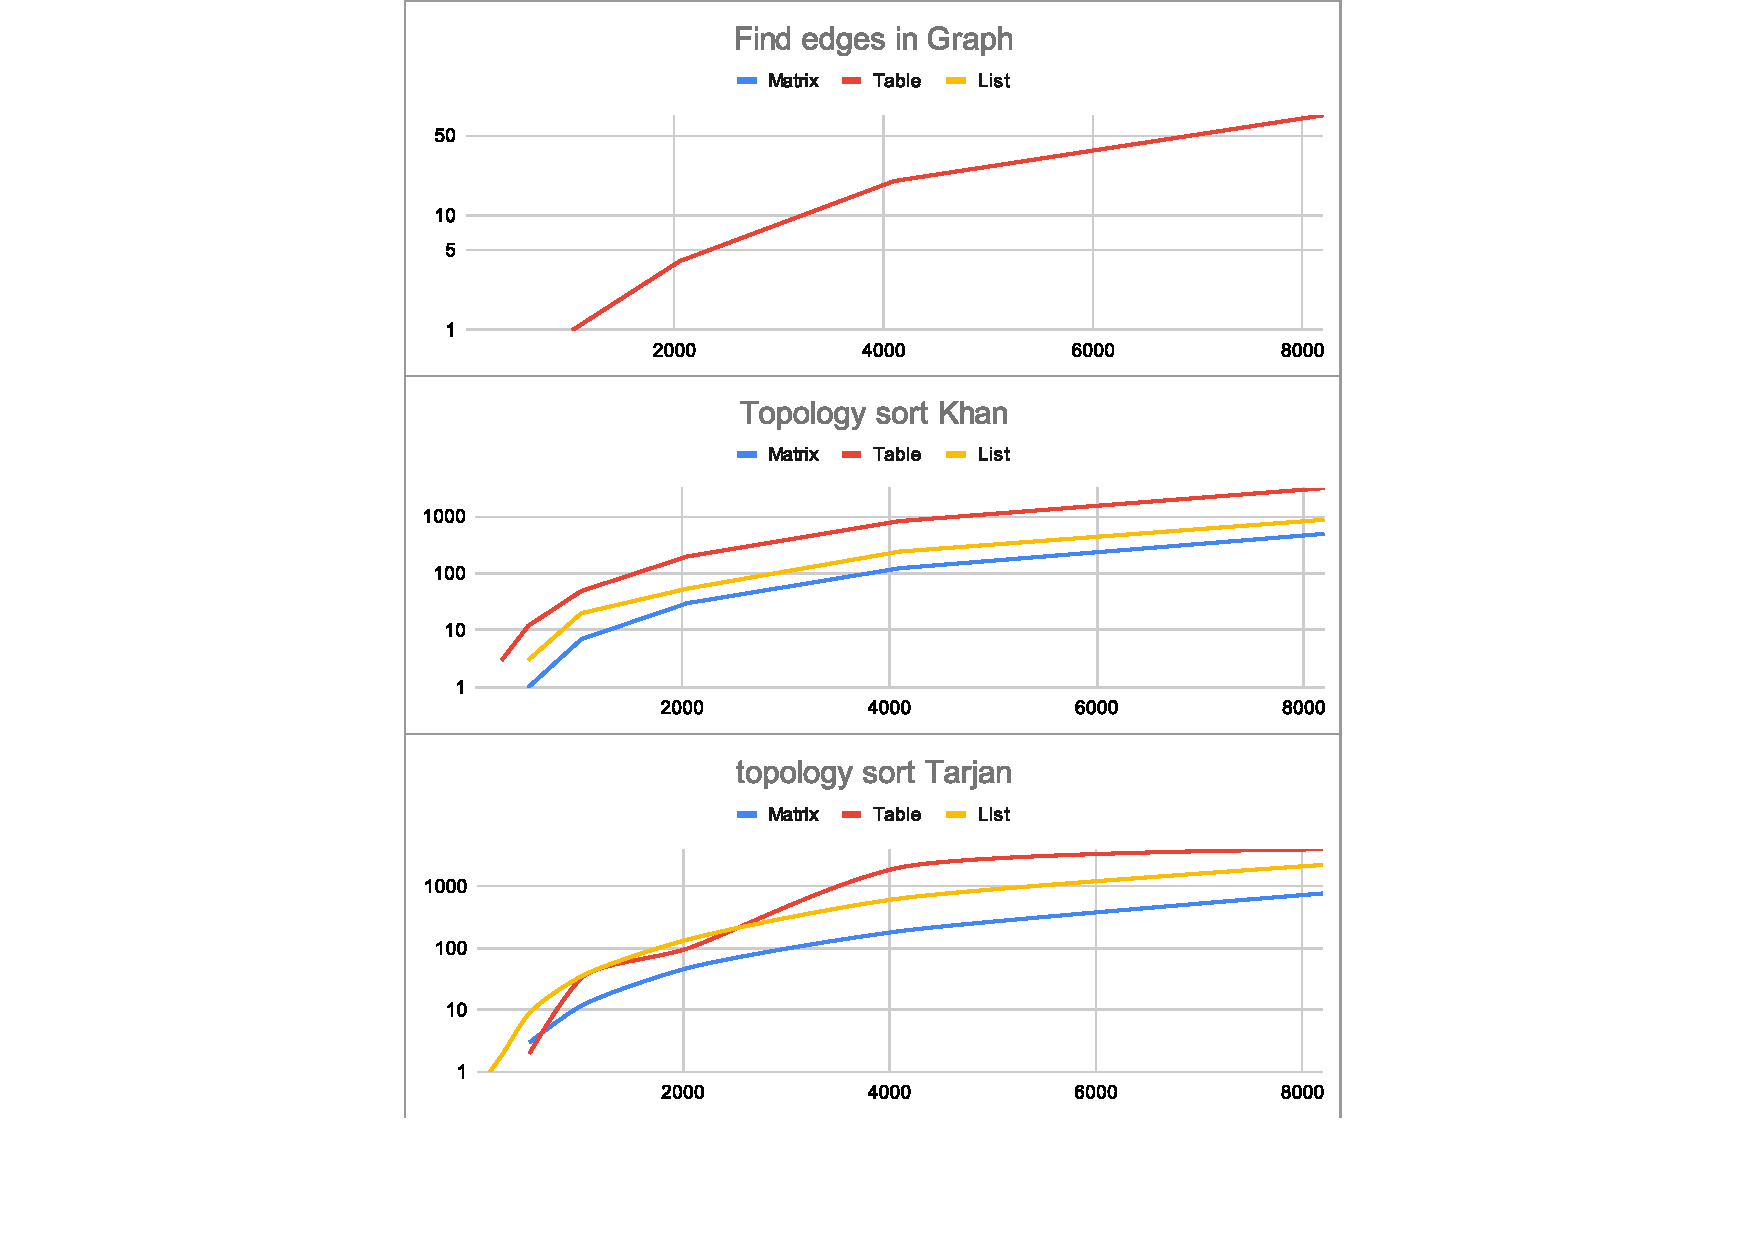
\includegraphics[width=\linewidth]{wykresy_logarytmiczna.pdf}

\end{center}

\section{Podsumowanie: }

Nauczyłem sie

\begin{enumerate}

	\item
	      Generować grafy.
	\item
		  Implementowac algorytmy ktore operuja na tych strukturach.
	\item
		  O grafach jako strukturach danych.
	\item
		  Jak zaimplementować algorytmy BFS i DFS.
	\item
		  Jak znajdowac krawedzie w grafach.
    \item
    	      Wypisywania na ekran.
  	\item
  		  Implementować algorytmy grafowe dla różnych reprezentacji maszynowych grafów.

\end{enumerate}

\begin{center}

\tableofcontents

\end{center}

\end{document}